\chapter{Application 2: Repository of Influencers for Content Recommendation}\label{chap:ch7}
\section{Introduction}

As discussed in previous chapters, a repository of location-aware influencers may be of interest for content recommendation and for studying location related communities from influencer's followers. This chapter describes the repository collected as part of this research, the features, and the visualization we employ. The repository consists of over three hundred thousand verified influencers that are tracked by \emph{@verified}. For each user, the location information, time, and language features are recorded as was described in chapters 2, 5, and 6, respectively. Additionally, other demographics such as gender and race are considered. %Such a repository could be used for (i) content recommendation, (ii) to build communities around the followers of influencers that are known to serve a specific geographic location, and other applications. 

\section{Related Research}
Popular variables associated with demographics are geographical location [\ref{appendix:1.3}], age [\ref{appendix:4.2}], gender [\ref{appendix:4.3}], education [\ref{appendix:4.4}, \ref{appendix:4.5}], income [\ref{appendix:4.6}], ethnicity [\ref{appendix:4.7}], and others. Typically, due to privacy concerns, these variables are not specifically stated. However, by fusing information with other sources, it is possible to characterize a group of users with a certain level of confidence. For example from the US Census Bureau's Genealogy Project which publishes the frequency of popular surnames with their distribution per race/ethnicity, it is possible to characterize the percent of users that belong to a certain ethnic group [\ref{appendix:4.7}]. A lot of the approaches deal with English-speakers [\ref{appendix:4.8}].

Many additional variables may be inferred from online connections a user has that apply to any language. For example followers of @ESPN and @SportsCenter are more likely to be male, followers of @PlayStation are more likely to be kids, and followers of @ParentsMagazine are likely to have kids [\ref{appendix:4.9}]. Political orientation may be discovered by whether the user is connected to known political representatives [\ref{appendix:4.10}]. Timezone and language can be used for differentiating between countries. Our goal is to focus on those demographic features that can be used to characterize a large portion of the global population. Our repository focuses on self-reported location, gender, race, language, and time of the day their account was created. 

\section{Setting up the Repository}

Implementation utilized Ubuntu 16.04 as the OS, Python 3.5 as the programming language, and MongoDB 3.6.5 as the NoSQL database. %The repository is stored in folders for MongoDB and Eclipse workbench. An instance of MongoDB and Eclipse simply need to point to the folders. For example, on Ubuntu, the command: mongod --dbpath `path' would point MongoDB to a specific folder. Specific Python libraries such as pymongo for interfacing with MongoDB are installed via pip. 
ElasticSearch and Kibana were used to search and visualize data of interest.

\begin{figure}[htbp]
\centerline{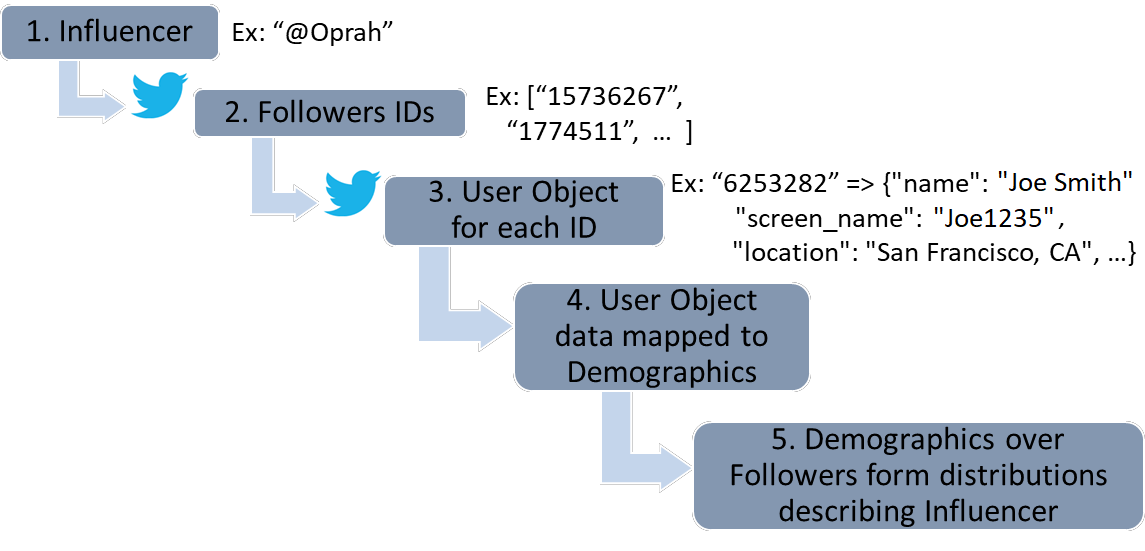
\includegraphics[width=4in]{Fig1.png}}
\caption{Collection Process.}
\label{fig_ch7_1}
\end{figure}

Fig. \ref{fig_ch7_1} illustrates the collection process for a single Twitter influencer. %The repository covers all of the Twitter influencers verified by Twitter. 
Each component from Fig. \ref{fig_ch7_1} is described below.

\begin{itemize}
\item Influencer to Follower IDs: influencers are identified from @verified. For each influencer, up to 5000 followers are collected. %We have seen that typically around 500 followers form a large enough sample to reason about influencer's demographics (for this reason and due to Twitter API limits for many influencers it is enough to collect at most 5000 followers). The connections between influencer to follower are stored in Twitter{\_}Connections database.

\item IDs to User Objects: Fig \ref{fig_ch7_2} is a Snapshot of our database. Database stores all followers and all influencers collected in tables `userInfo' and `followerInfo' respectively. Example of User Object from userInfo table shown in Fig \ref{fig_ch7_3}.

\begin{figure}[htbp]
\centerline{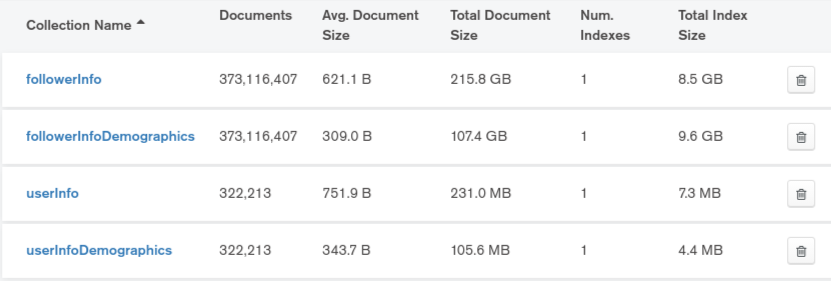
\includegraphics[width=5in]{Fig2.png}}
\caption[Database holding Twitter User Objects]{Database holding Twitter User Objects for 322 thousand influencers and 373 million followers.}
\label{fig_ch7_2}
\end{figure}

\begin{figure}[htbp]
\centerline{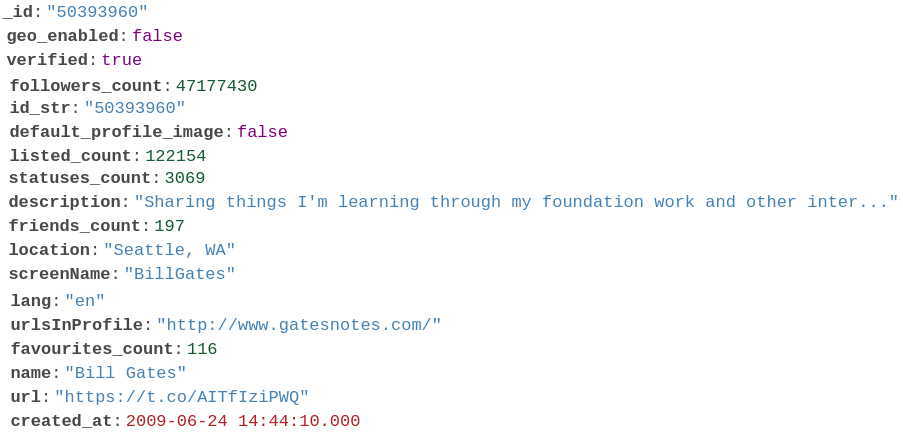
\includegraphics[width=5in]{Fig3.png}}
\caption{Example fields for Twitter User Object corresponding to @BillGates}
\label{fig_ch7_3}
\end{figure}

\item User Object to Demographics: User's textual location is matched against GeoNames city/country pairs, the self-reported name is matched against names with known gender and ethnicity. The associated demographic info, for all followers and all influencers, is stored in tables `userInfoDemographics' and `followerInfoDemographics', respectively. If gender is present it is given by `pctFemale' and `pctMale'; race given by `pctapi': Asian, `pctblack': African American, `pctwhite': Caucasian, `pcthispanic': Hispanic. %For example, for \emph{@kobebryant} the name Kobe is 96.87\% male and the last name Bryant is 58.46\% Caucasian and 35.58\% African American. The details for how these are computed are given later on.

\item Demographics to Distributions: all influencer's followers with gender, race, location, language, time information are used to form corresponding frequency distributions. These distributions can then be used to understand the influencer's influence over the ordinary population by analyzing the percent of influencer's followers within certain gender, language, and so on. %These distributions are stored in DB: `twitter{\_}demographics{\_}across{\_}followers'. 
%As an example the top ten influencers out of 3104 influencers with over 50.0\% of their followers speaking the Turkish language shown in Fig \ref{fig_ch7_4}.
\end{itemize}

\iffalse
\begin{figure}[htbp]
\centerline{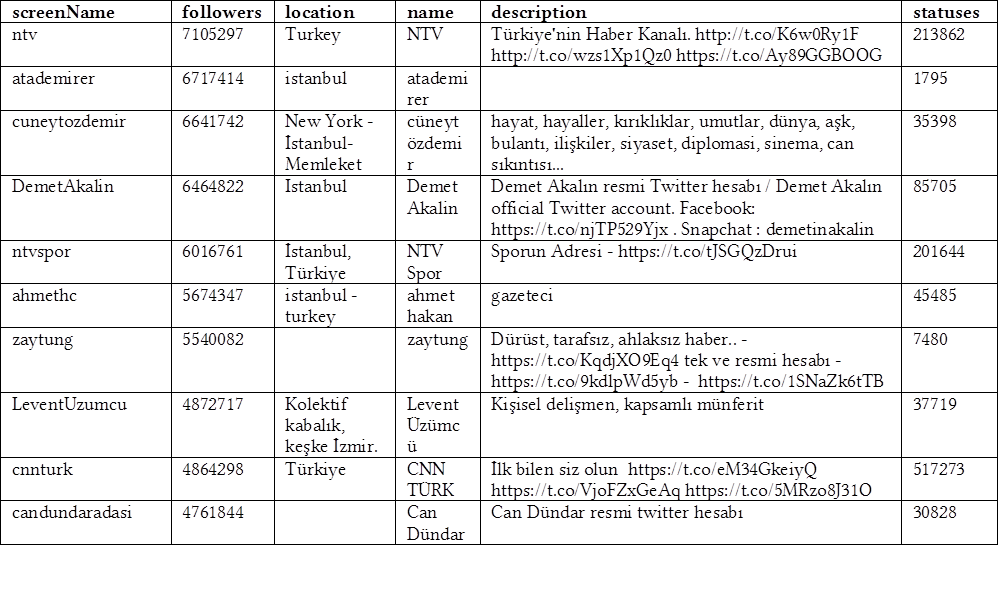
\includegraphics[width=5.4in]{Fig7.png}}
\caption[Top influencers of Turkish speakers]{Top 10 Influencers with mostly Turkish speaking audience.}
\label{fig_ch7_4}
\end{figure}
\fi

ElasticSearch is utilized for loading and exploring data that is relevant to a specific scenario. Thus while MongoDB holds all of the data, ElasticSearch is used to search for a specific demographic. The end-user can utilize the Kibana visualization to form custom queries and zoom in and out on the map. Fig. \ref{fig_ch7_5} shows the visualization dashboard over followers for influencer @CNNEE (CNN Espanol) (similarly any one of the 320K influencers can be visualized).

\begin{figure}[htbp]
\centerline{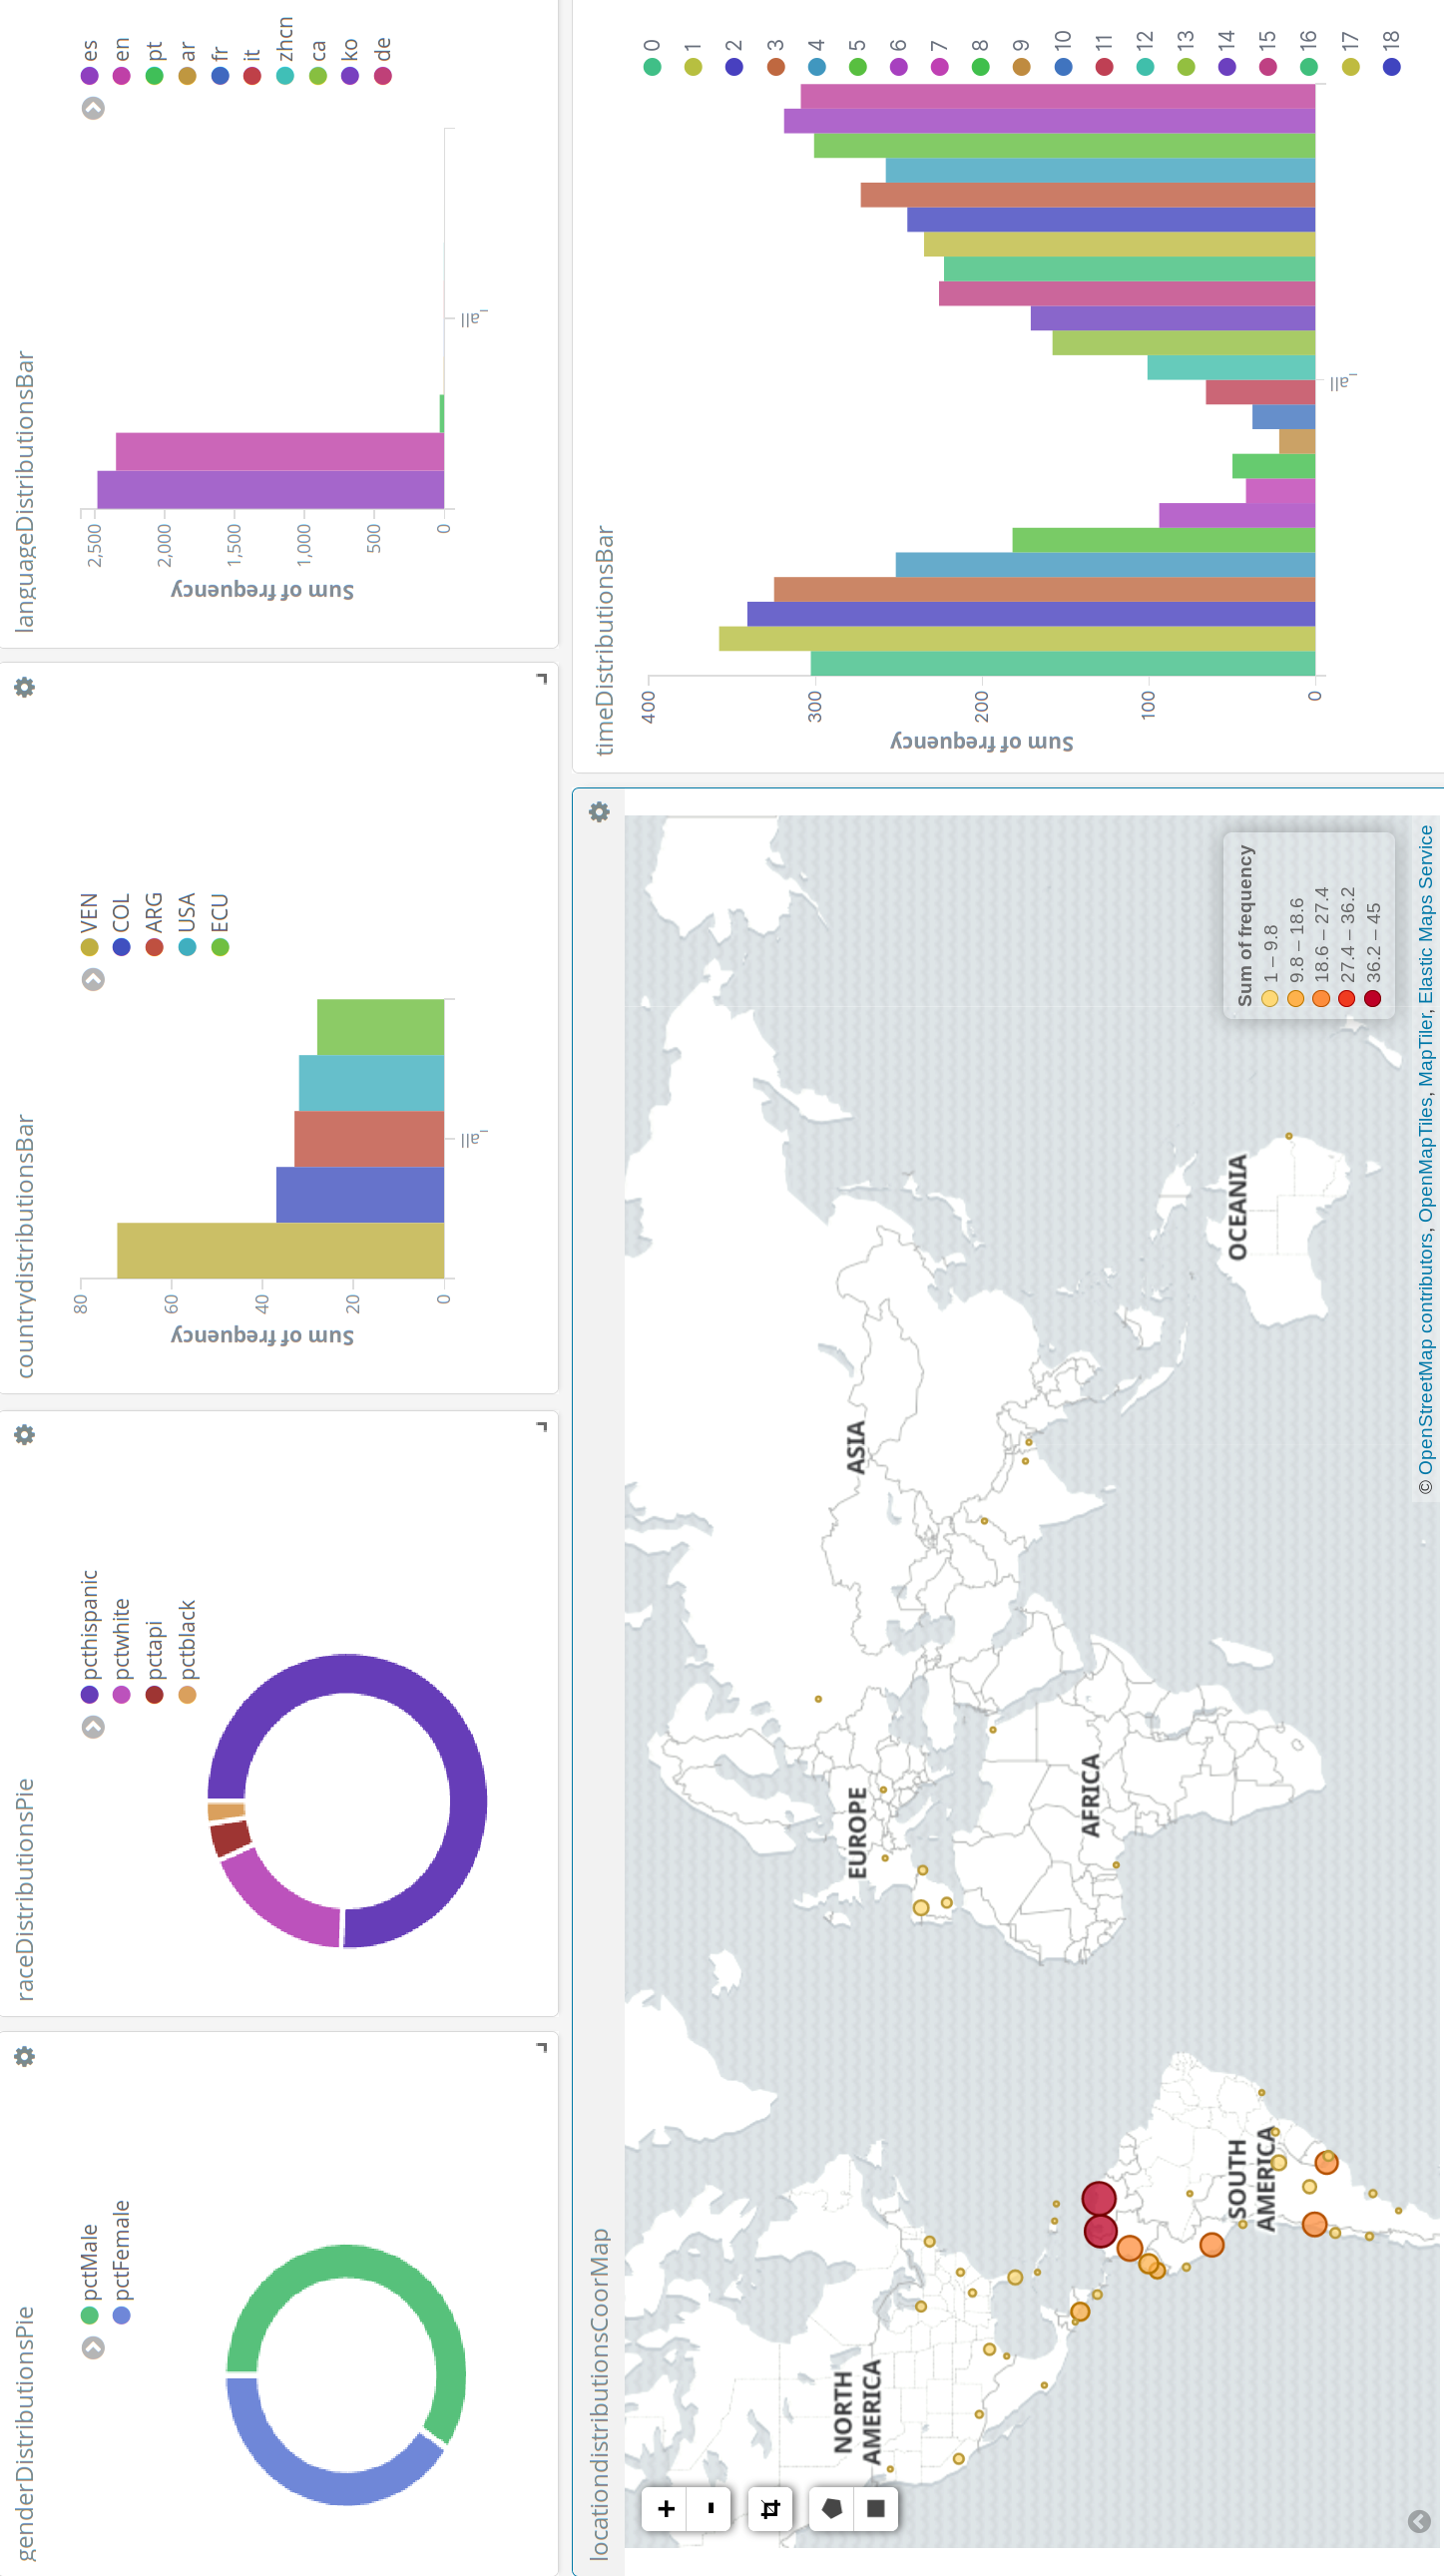
\includegraphics[width=4in]{Fig10.png}}
\caption[Visualizing influence by demographic]{Visualizing influence by demographic. Understanding the influence of @CNNEE.}
\label{fig_ch7_5}
\end{figure}

\section{Features used in Repository}
\subsection{Location}
Chapter 2 described an approach for geocoding a user's textual location. The rules of the classifier developed illustrated that it is important to consider whether a location that is matched contains both the city and state as this is less ambiguous than a city name by itself. Because Google's geocoder is limited, by the number of API calls it can freely make daily, we focused on matching locations that contain a known city/state or city/country for a high precision/low recall solution. For our task, it is better to focus on high precision locations given that verified influencers typically have thousands of followers which generally provides a large enough sample (as seen in section 4.7.2) to accurately pinpoint the influencer's city location.

%Utilizing cities from GeoNames with a population over five thousand\footnote{http://download.geonames.org/export/dump/cities5000.zip}. Country info such as iso codes, fips codes, languages, capital, are also collected from GeoNames\footnote{http://download.geonames.org/export/dump/countryInfo.txt}. 
GeoNames data is processed by (i) verifying each city entry to have a population above five thousand (806 entries were filtered out) and (ii) removing duplicate entries that refer to the same city by taking the most recent entry or one with the highest population (981 entries removed).

\begin{table}
\small
\caption{Countries with most and least cities from GeoNames}
\label{table_1_app2}
\begin{center}
\begin{tabular}{|c|c|c|c|}
\multicolumn{2}{c}{\bfseries Top 20 Country to City} &
\multicolumn{2}{c}{\bfseries Bottom 20 Country to City}\\
\hline
United States & 7113 & Saint Martin & 1 \\
\hline
India & 3189 & Sao Tome and Principe & 1 \\
\hline
Germany & 2780 & Guernsey & 1 \\
\hline
Russia & 2525 & Saint Kitts and Nevis & 1 \\
\hline
France & 1972 & Saint Barthelemy & 1 \\
\hline
Italy & 1919 & Saint Pierre and Miquelon & 1 \\
\hline
Brazil & 1854 & Jersey & 1 \\
\hline
Mexico & 1725 & Seychelles & 1 \\
\hline
United Kingdom & 1603 & Cook Islands & 1 \\
\hline
Spain & 1302 & Tonga & 1 \\
\hline
Philippines & 1160 & British Virgin Islands & 1 \\
\hline
China & 842 & Gibraltar & 1 \\
\hline
Australia & 816 & Palau & 1 \\
\hline
Romania & 755 & Grenada & 1 \\
\hline
Japan & 739 & Faroe Islands & 1 \\
\hline
Turkey & 714 & Antigua and Barbuda & 1 \\
\hline
Poland & 661 & Dominica & 1 \\
\hline
Ukraine & 641 & Barbados & 1 \\
\hline
Netherlands & 484 & Aland Islands & 1 \\
\hline
Colombia & 484 & Macao & 1 \\
\hline
\end{tabular}
\end{center}
\end{table}

For each city, the City + Country Name, Country ISO, Country FIPS, and Country ISO3 are recorded as query strings. For example, for London UK these are the possible strings: `londongbr', `londonuk', `londonunitedkingdom', `londongb'. For the United States, we also search for City + State Name or State Abbreviation; for example `uticany', `uticanewyork'. The country name is utilized for cities with a population over 100K: `syracuseunitedstates', `syracuseus', `syracuseusa' (fips and iso equal in this example). This is done for cities where there is no other city with population over 100K (example `arlingtonus' is not allowed since it can refer to Arlington TX or Arlington VA which both have a population over 100K). There are also cities such as New York City which have `City' as part of the name, but that users may choose not to spell out; we allow city name variations with following tokens removed: `municipality', `village', `city', `charter', `township', and `town'. %So for New York NY USA the possibilities are: newyorkusa, newyorkcityny (with and without `city'). Thus in our representation there are a total of ten string representations for New York NY USA: newyorkusa, newyorkcityunitedstates, newyorkcityus, newyorkcitynewyork, newyorkcityny, newyorkcityusa, newyorkny, newyorkus, newyorknewyork, and newyorkunitedstates. 

In all, there were 47119 unique cities and 156037 corresponding representations. Each follower's self-reported location is turned to lowercase with punctuation and whitespace stripped out. Follower's preprocessed location is utilized if it matches one of the 156037 corresponding representations. Table \ref{table_1_app2} shows the number of unique cities associated with each country. 

In all 225 countries are represented. For each influencer, locations over all followers are used to form a location distribution. The cities in location distribution can be aggregated to generate a country distribution. Location and country distributions are used to identify influencers serving a specific region of the world.

\subsection{Gender}
Social Security Administration (SSA) provides popular female and male names\footnote{https://www.ssa.gov/oact/babynames/names.zip}. The data contains the name, gender, and frequency. A specific name can be used as a female and a male example from file: Emma, F, 19738 and Emma, M, 14. The frequency for gender divided by total frequency gives a percentage for how likely a particular name is to be male vs. female. Given frequencies for Emma, P(Emma, F) = 99.93\% and P(Emma, M) = 0.071\% as probabilities for female and male, respectively. Some names are on the borderline: Temiloluwa 55\%, Carroll 45.5\%, and Arley 57.3\% (male probability). 

This dataset consisted of 29910 names. For each Twitter follower, the first token of the name field is utilized. The token is converted to lowercase with punctuation stripped out. If it is contained within the names dataset then it is assigned a gender probability. For each influencer, the male and female probabilities over followers are added up and divided by the number of followers with name information.

\subsection{Ethnicity}
The Census Bureau identifies the last name to race mapping. The 2010 dataset provides Surnames Occurring 100 or more times with 162254 surnames\footnote{https://www2.census.gov/topics/genealogy/2010surnames/names.zip}. We use the following four race categories: Non-Hispanic White Alone (White), Non-Hispanic Black or African American Alone (Black), Non-Hispanic Asian and Native Hawaiian and Other Pacific Islander Alone (Asian) and Hispanic or Latino origin (Hispanic) (there are two more categories, but those have too few data points, see reference [\ref{appendix:4.12}]).
%Non-Hispanic White Alone, Non-Hispanic Black or African American Alone, Non-Hispanic American Indian and Alaska Native Alone, Non-Hispanic Asian and Native Hawaiian and Other Pacific Islander Alone, Non-Hispanic Two or More Races, and Hispanic or Latino origin. Method focuses on four categories: Non-Hispanic White Alone (Pctwhite), Non-Hispanic Black or African American Alone (Pctblack), Non-Hispanic Asian and Native Hawaiian and Other Pacific Islander Alone (Pctapi) and Hispanic or Latino origin (Pcthispanic). This is inspired by reference [\ref{appendix:4.12}] where authors also focus on these four categories (other categories such as Alaskan Native have too few data points). 
For each Twitter follower, if the self-reported name contains two tokens then the second token of the name field is utilized. The token is converted to lowercase with punctuation stripped out. If it is contained within the surnames dataset then it is utilized. For each influencer, the ethnicity probabilities over followers are added up and divided by the number of followers with ethnicity information. 

\subsection{Time and Language}

\begin{table}
\small
\caption{Top 20 Languages Across the Dataset}
\label{table_2_app2}
\begin{center}
\begin{tabular}{|c|c|c|}
\hline
\bfseries language code& \bfseries follower count& \bfseries overall percent\\
\hline
en&244313028&64.7\\
\hline
es&33680216&8.92\\
\hline
ja&13899866&3.68\\
\hline
ar&11024275&2.92\\
\hline
pt&10550007&2.79\\
\hline
fr&10374538&2.75\\
\hline
tr&9024648&2.39\\
\hline
ru&7717812&2.04\\
\hline
engb&5279311&1.4\\
\hline
none&4495906&1.19\\
\hline
id&4373498&1.16\\
\hline
de&4154066&1.1\\
\hline
it&3094860&0.82\\
\hline
zhcn&2942235&0.78\\
\hline
nl&1965084&0.52\\
\hline
ko&1340514&0.35\\
\hline
vi&1154730&0.31\\
\hline
pl&959457&0.25\\
\hline
th&933313&0.25\\
\hline
sv&753957&0.2\\
\hline
zhtw&613812&0.16\\
\hline
\end{tabular}
\end{center}
\end{table}

The time distribution over influencer's followers is generated as described in Section 5.2. The language field is available for 98.81\% of users. %On Twitter users specify the language that they would want their Twitter dashboard to display in. 
Table \ref{table_2_app2} shows the top 20 languages over 373116407 users. The table shows that about 64.7\% of users prefer English, 8.92\% prefer Spanish, 3.68\%  prefer Japanese, and so on. %Only 1.19\% of users have no info for this field. 
For each influencer, the ratio of followers preferring a specific language is recorded. Influencers who target a specific country such as Spain are expected to have an above average number of Spanish speakers.

\subsection{DBPedia}

\iffalse
\begin{figure}[htbp]
\centerline{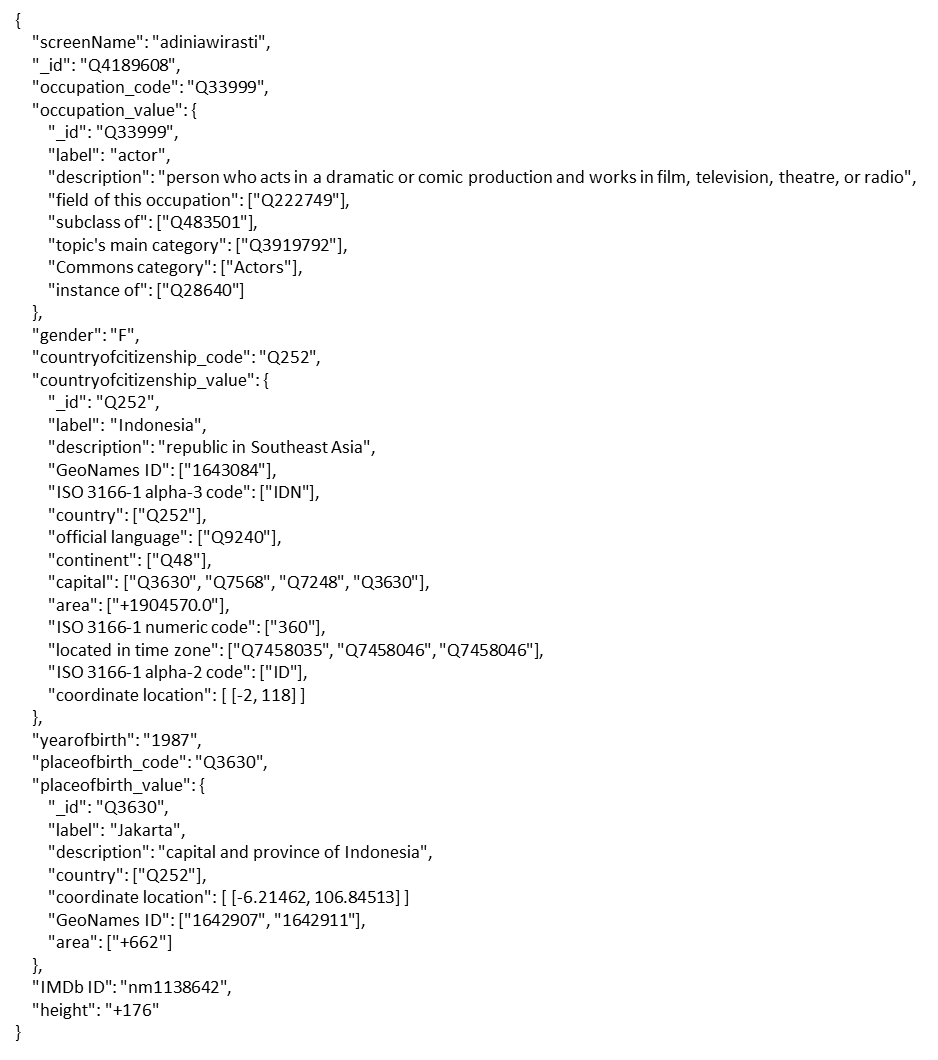
\includegraphics[width=6in]{Fig11.png}}
\caption[DBPedia Data]{Example of additional data brought via DBPedia.}
\label{fig_ch7_6}
\end{figure}
\fi

DBPedia is a large publicly available resource that is used for leveraging external data related to Twitter users. We are interested in those DBPedia pages that have a matching Twitter screenname. Sometimes this will be part of infobox data, other times this data can be predicted. Reference [\ref{appendix:4.15}] is an example of a recent paper that attempts to match DBPedia pages to Twitter screennames. For training and test data, they try the top-ranked Twitter profile (if any) returned by Twitter when queried with the DBPedia entity name. 893,446 DBPedia entities were matched to 630,767 Twitter candidates and a Deep Neural Net (DNN) used to align 169,748 of these. For evaluation, their gold standard is made of those DBpedia pages where the Twitter screenname is explicitly stated consisting of 56,133 alignments from English DBpedia entities (40,967 persons, 15,166 organizations). 

We utilize SocialLink latest Gold and latest predicted mappings that had a score of 0.75 or greater (75\% or higher confidence). Out of these influencers, 44450 appear in our dataset (12,771 from gold and 36,029 from predicted, some influencers appear in both lists).

DBPedia uses a Virtuoso RDF triple store that requires SPARQL queries. If a page exists on Wikipedia such as: `https://en.wikipedia.org/wiki/Oprah{\_}Winfrey' it is also available on DBPedia `http://dbpedia.org/page/Oprah{\_}Winfrey' (unique id being `Oprah{\_}Winfrey'). A Python client library called Wikidata\footnote{https://github.com/dahlia/wikidata} was used.

Each DBPedia page is represented by Q{\#}. Each result contains the label, description, claims, and references. The first step was to collect all claims for each DBPedia page that had a link to a Twitter influencer. The frequency of all unique claims was recorded with some of the items of interest from Table \ref{table_3_app2}. 

\begin{table}
\small
\caption{DBPedia Categories of Interest}
\label{table_3_app2}
\begin{center}
\begin{tabular}{|c|c|c|}
\hline
\bfseries DBPedia ID & \bfseries label & \bfseries Number of Values\\
\hline
P27 & country of citizenship & 224\\
\hline
P569 & date of birth & 9245\\
\hline
P172 & ethnic group & 213\\
\hline
P1412 & languages spoken, written or signed & 141\\
\hline
P21 & sex or gender & 8\\
\hline
P19 & place of birth & 9245\\
\hline
P140 & religion & 124\\
\hline
P69 & educated at & 5660\\
\hline
P735 & given name & 6222\\
\hline
P734 & family name & 10420\\
\hline
P106 & occupation & 1207\\
\hline
P641 & sport & 194\\
\hline
P54 & member of sports team & 5143\\
\hline
P136 & genre & 649\\
\hline
\end{tabular}
\end{center}
\end{table}

Each item listed points to a separate DBPedia page. For example, there are is a separate page for each country, where each page provides additional information such as the country's coordinates, population, inception date, and other information. In this way, for each influencer, we attempt to collect all categories shown in Table \ref{table_3_app2} and then for each category we collect additional information that characterizes the category. This leads to a rich set of additional data available for influencers that are popular enough to be described on Wikipedia. %Fig 5.6 shows a snapshot of brought in data showing an influencer's occupation, place of birth, and country of citizenship. All items marked with QQ{\#} refer to DBPedia pages from which more info can be extracted.

\section{Example Rankings by Demographic Group}

This section illustrates how the repository can be used for content recommendation for a certain demographic; where the demographic is based on gender, ethnicity, language, location, or a combination of these. 

For each demographic feature, our approach is to (i) for each influencer to record the percent of followers that fall into the demographic, (ii) record the average and standard deviation of the percent across all influencers, and (iii) set threshold equal to average plus one standard deviation. Table \ref{table_summaryFeatures_app2} shows the computed thresholds for demographic features related to gender and ethnicity.

\begin{table}
\small
\caption[Demographic Feature Ranges for Gender and Ethnicity]{For each Feature, the Average and Standard Deviation are computed across 320K influencers. This sets a threshold for influencers that capture above the average demographic. Number of influencers recommended for each demographic feature shown in last column.}
\label{table_summaryFeatures_app2}
\begin{center}
\begin{tabular}{|c|c|c|c|c|}
\hline
\bfseries Feature & \bfseries AVG & \bfseries STD & \bfseries T = AVG+STD & \bfseries Influencers\\
\hline
Gender Male & 61.69\% & 16.37\% & 78.06\% & 61988 \\
\hline
Gender Female & 38.34\% & 16.35\% & 54.69\% & 46935 \\
\hline
Ethnicity White & 60.39\% & 17.89\% & 78.28\% & 19179 \\
\hline
Ethnicity Black & 10.95\% & 5.09\% & 16.04\% & 26256 \\
\hline
Ethnicity Hispanic & 13.65\% & 16.26\% & 29.92\% & 33010 \\
\hline
Ethnicity Asian & 11.72\% & 15.03\% & 26.75\% & 33300 \\
\hline
\end{tabular}
\end{center}
\end{table}

\begin{table}
\small
\caption[Top Influencers with male vs. female audience]{Top 10 Most Popular Influencers for each Gender.}
\label{table_4_app2}
\begin{center}
\begin{tabular}{|c|c|c|c|}
\multicolumn{4}{c}{\bfseries Top 10 Influencers with over 78.06\% Followers being male}\\
\hline
\bfseries screenName & \bfseries followers & \bfseries name & \bfseries {\%}Male\\
\hline
narendramodi & 47235007 &Chowkidar Narendra Modi& 81.39 \\
\hline
SrBachchan & 37091473 &Amitabh Bachchan& 80.41\\
\hline
BeingSalmanKhan & 36816795 & Salman Khan & 81.18\\
\hline
SportsCenter & 35437313 & SportsCenter & 78.58\\
\hline
realmadrid & 31984155 & Real Madrid C.F. & 85.34\\
\hline
akshaykumar & 30511248 & Akshay Kumar  & 78.97\\
\hline
FCBarcelona & 29627195 & FC Barcelona & 85.0\\
\hline
imVkohli & 29436203 & Virat Kohli & 83.95\\
\hline
sachin{\_}rt & 29057313 & Sachin Tendulkar & 84.32\\
\hline
PMOIndia & 28895265 & PMO India & 83.17\\
\hline
\multicolumn{4}{c}{}\\
\multicolumn{4}{c}{\bfseries Top 10 Influencers with over 54.69\% Followers being female}\\
\hline
\bfseries screenName & \bfseries followers & \bfseries name & \bfseries{\%}Female\\
\hline
justinbieber & 105481835 & Justin Bieber & 64.03\\
\hline
TheEllenShow & 77630706 & Ellen DeGeneres &62.09\\
\hline
ArianaGrande & 62676030 & Ariana Grande & 59.2\\
\hline
KimKardashian & 60662411 &Kim Kardashian West& 57.68\\
\hline
selenagomez & 57579185 & Selena Gomez & 58.51\\
\hline
jimmyfallon & 51109039& jimmy fallon & 55.94\\
\hline
MileyCyrus & 42505219 & Miley Ray Cyrus & 58.68\\
\hline
NiallOfficial & 39292796 & Niall Horan & 62.67\\
\hline
Harry{\_}Styles & 33315825 & Harry Styles. & 79.25\\
\hline
Louis{\_}Tomlinson & 33232768 & Louis Tomlinson & 67.75\\
\hline
\end{tabular}
\end{center}
\end{table}

\iffalse
\begin{table}
\small
\caption[Top Influencers with male vs. female audience]{Top 10 Most Popular Influencers for each Gender.}
\label{table_4_app2}
\begin{center}
\begin{tabular}{|c|c|c|c|c|}
\multicolumn{5}{c}{\bfseries Top 10 Influencers with over 78.06\% Followers being male}\\
\hline
\bfseries screenName & \bfseries followers & \bfseries profile location & \bfseries name & \bfseries {\%}Male\\
\hline
narendramodi & 47235007 & India &Chowkidar Narendra Modi& 81.39 \\
\hline
SrBachchan & 37091473 & Mumbai, India &Amitabh Bachchan& 80.41\\
\hline
BeingSalmanKhan & 36816795 & MUMBAI & Salman Khan & 81.18\\
\hline
SportsCenter & 35437313 &  & SportsCenter & 78.58\\
\hline
realmadrid & 31984155 & Madrid, Spain & Real Madrid C.F. & 85.34\\
\hline
akshaykumar & 30511248 &  & Akshay Kumar  & 78.97\\
\hline
FCBarcelona & 29627195 & Barcelona & FC Barcelona & 85.0\\
\hline
imVkohli & 29436203 &  & Virat Kohli & 83.95\\
\hline
sachin{\_}rt & 29057313 &UT: 18.986431,72.823769& Sachin Tendulkar & 84.32\\
\hline
PMOIndia & 28895265 & India  & PMO India & 83.17\\
\hline
\multicolumn{5}{c}{}\\
\multicolumn{5}{c}{\bfseries Top 10 Influencers with over 54.69\% Followers being female}\\
\hline
\bfseries screenName & \bfseries followers & \bfseries profile location & \bfseries name & \bfseries{\%}Female\\
\hline
justinbieber & 105481835 &  & Justin Bieber & 64.03\\
\hline
TheEllenShow & 77630706 & California & Ellen DeGeneres &62.09\\
\hline
ArianaGrande & 62676030 & honeymoon ave & Ariana Grande & 59.2\\
\hline
KimKardashian & 60662411 &   &Kim Kardashian West& 57.68\\
\hline
selenagomez & 57579185 & Los Angeles & Selena Gomez & 58.51\\
\hline
jimmyfallon & 51109039 &New York,New York& jimmy fallon & 55.94\\
\hline
MileyCyrus & 42505219 &  & Miley Ray Cyrus & 58.68\\
\hline
NiallOfficial & 39292796 &Mullingar,Westmeath,Ireland& Niall Horan & 62.67\\
\hline
Harry{\_}Styles & 33315825 &  & Harry Styles. & 79.25\\
\hline
Louis{\_}Tomlinson & 33232768 & Doncaster & Louis Tomlinson & 67.75\\
\hline
\end{tabular}
\end{center}
\end{table}
\fi

\noindent\textbf{Gender}-- The gender was computed for 185078761 out of 373116407 (49.6\%) of users. Across all users 57.6\% were male. Across all influencers on average 61.69\% of followers were male with a standard deviation of 16.37\% (threshold = 61.69\%+16.37\% = 78.07\%). The last column shows that there were 61988 influencers whose audience is over 78.07\% male. Top ten influencers exceeding this threshold and ordered by the number of followers shown in Table \ref{table_4_app2} (top). Similarly, 46935 influencers whose audience is over 54.69\% female, with the corresponding top ten influencers shown in Table \ref{table_4_app2} (bottom). 

\noindent\textbf{Ethnicity}-- For ethnicity, 125780191 out of 373116407 (33.71\%) users had, as a second token in their name, a surname that maps to a known ethnicity. Of these 56.54\% were White, 18.21\% Hispanic, 13.98\% Asian, and 10.27\% Black. Table \ref{table_summaryFeatures_app2} shows the computed thresholds for each ethnicity across influencers' followers. Using these thresholds the top influencers for each ethnicity shown in Table \ref{table_6_app2}. %Note: Hindus are not broken out as a separate ethnicity and as a result are associated with Asians (India falls into South Asia), for this reason some influencers with Asian audience are from India.

\begin{table}
\small
\caption[Top Influencers for each Ethnicity]{Most Popular Influencers for each Ethnicity.}
\label{table_6_app2}
\begin{center}
\begin{tabular}{|c|c|c|c|}
\multicolumn{4}{c}{\bfseries Top 6 Influencers with over 78.28\% Followers being Caucasian}\\
\hline
\bfseries screenName & \bfseries followers & \bfseries name & \bfseries {\%}Caucasian\\
\hline
lorenzojova & 3819516 & Lorenzo Jovanotti & 79.13 \\
\hline
repubblica & 2857050 & la Repubblica & 78.6 \\
\hline
SPIEGELONLINE & 2529707 & SPIEGEL ONLINE & 78.76 \\
\hline
beppe{\_}grillo & 2470978 & Beppe Grillo & 79.78 \\
\hline
MarroneEmma & 2469369 & Emma Marrone & 80.44 \\
\hline
radiodeejay & 2278769 & Radio Deejay & 81.63 \\
%\hline
%officiallyjoko & 2204608 & joko winterscheidt & 82.17 \\
%\hline
%redazioneiene & 2199359 & Le Iene & 81.82 \\
%\hline
%ligabue & 2177024 & Luciano Ligabue & 81.38 \\
%\hline
%m{\_}hunziker & 2168051 & Michelle Hunziker & 79.52 \\
\hline
\multicolumn{4}{c}{}\\
\multicolumn{4}{c}{\bfseries Top 6 Influencers with over 16.04\% Followers being African American}\\
\hline
\bfseries screenName & \bfseries followers & \bfseries name & \bfseries {\%}Black\\
\hline
Oprah & 42164712 & Oprah Winfrey & 16.51 \\
\hline
KevinHart4real & 35194359 & Kevin Hart & 16.12 \\
\hline
LilTunechi & 34235040 & Lil Wayne WEEZY F & 19.82 \\
\hline
wizkhalifa & 34028999 & Wiz Khalifa & 16.51 \\
\hline
chrisbrown & 30245761 & Chris Brown & 19.24 \\
\hline
aliciakeys & 30023640 & Alicia Keys & 18.01 \\
%\hline
%andresiniesta8 & 24127051 & Andrés Iniesta & 16.52 \\
%\hline
%MesutOzil1088 & 24016907 & Mesut Özil & 18.18 \\
%\hline
%NICKIMINAJ & 20455827 & QUEEN & 17.63 \\
%\hline
%premierleague & 19432386 & Premier League & 18.75 \\
\hline
\multicolumn{4}{c}{}\\
\multicolumn{4}{c}{\bfseries Top 6 Influencers with over 29.92\% Followers being Hispanic}\\
\hline
\bfseries screenName & \bfseries followers & \bfseries name & \bfseries {\%}Hispanic\\
\hline
shakira & 51127526 & Shakira & 35.82 \\
\hline
Louis{\_}Tomlinson & 33232768 & Louis Tomlinson & 33.29 \\
\hline
realmadrid & 31984155 & Real Madrid C.F. & 31.11 \\
\hline
pitbull & 26128582 & Pitbull & 31.71 \\
\hline
ricky{\_}martin & 20383994 & Ricky Martin & 56.29 \\
\hline
AlejandroSanz & 19516691 & Alejandro Sanz & 71.78 \\
%\hline
%3gerardpique & 19243546 & Gerard Piqué & 40.37 \\
%\hline
%10Ronaldinho & 18624086 & Ronaldinho Gaúcho & 31.81 \\
%\hline
%jamesdrodriguez & 18181928 & James Rodríguez & 55.84 \\
%\hline
%DaniloGentili & 17316619 & Danilo Gentili & 32.13 \\
\hline
\multicolumn{4}{c}{}\\
\multicolumn{4}{c}{\bfseries Top 6 Influencers with over 26.75\% Followers being Asian}\\
\hline
\bfseries screenName & \bfseries followers & \bfseries name & \bfseries {\%}Asian\\
\hline
narendramodi & 47235007 & Chowkidar Narendra Modi & 78.17 \\
\hline
BillGates & 47177430 & Bill Gates & 33.24 \\
\hline
iamsrk & 38104866 & Shah Rukh Khan & 73.74 \\
\hline
SrBachchan & 37091473 &Amitabh Bachchan& 76.75 \\
\hline
BeingSalmanKhan & 36816795 & Salman Khan & 72.79 \\
\hline
akshaykumar & 30511248 & Akshay Kumar & 73.73 \\
\hline
%imVkohli & 29436203 & Virat Kohli & 75.84 \\
%\hline
%sachin{\_}rt & 29057313 & Sachin Tendulkar & 76.86 \\
%\hline
%PMOIndia & 28895265 & PMO India & 80.59 \\
%\hline
%deepikapadukone & 26090675 & Deepika Padukone & 75.99 \\
%\hline
\end{tabular}
\end{center}
\end{table}

\iffalse
\begin{table}
\scriptsize
\caption[Top Influencers of different ethnicity]{Top 10 Most Popular Influencers for each Ethnicity.}
\label{table_6_app2}
\begin{center}
\begin{tabular}{|c|c|c|c|c|}
\multicolumn{5}{c}{\bfseries Top 10 Influencers with over 78.28\% Followers being Caucasian}\\
\hline
\bfseries screenName & \bfseries followers & \bfseries profile location & \bfseries name & \bfseries {\%}Caucasian\\
\hline
lorenzojova & 3819516 &  & Lorenzo Jovanotti & 79.13 \\
\hline
repubblica & 2857050 & Rome, Italy & la Repubblica & 78.6 \\
\hline
SPIEGELONLINE & 2529707 & Hamburg, Germany & SPIEGEL ONLINE & 78.76 \\
\hline
beppe{\_}grillo & 2470978 & Genova, Italia & Beppe Grillo & 79.78 \\
\hline
MarroneEmma & 2469369 &  & Emma Marrone & 80.44 \\
\hline
radiodeejay & 2278769 & Italy & Radio Deejay & 81.63 \\
\hline
officiallyjoko & 2204608 & berlin...city & joko winterscheidt & 82.17 \\
\hline
redazioneiene & 2199359 & Milano & Le Iene & 81.82 \\
\hline
ligabue & 2177024 & Correggio (RE) & Luciano Ligabue & 81.38 \\
\hline
m{\_}hunziker & 2168051 & Italy & Michelle Hunziker & 79.52 \\
\hline
\multicolumn{5}{c}{}\\
\multicolumn{5}{c}{\bfseries Top 10 Influencers with over 16.04\% Followers being African American}\\
\hline
\bfseries screenName & \bfseries followers & \bfseries profile location & \bfseries name & \bfseries {\%}Black\\
\hline
Oprah & 42164712 &  & Oprah Winfrey & 16.51 \\
\hline
KevinHart4real & 35194359 & Philly/LA & Kevin Hart & 16.12 \\
\hline
LilTunechi & 34235040 &  & Lil Wayne WEEZY F & 19.82 \\
\hline
wizkhalifa & 34028999 & Pix Burgh & Wiz Khalifa & 16.51 \\
\hline
chrisbrown & 30245761 &  & Chris Brown & 19.24 \\
\hline
aliciakeys & 30023640 & New York City & Alicia Keys & 18.01 \\
\hline
andresiniesta8 & 24127051 & Barcelona & Andrés Iniesta & 16.52 \\
\hline
MesutOzil1088 & 24016907 & England & Mesut Özil & 18.18 \\
\hline
NICKIMINAJ & 20455827 & Q U E E N & QUEEN & 17.63 \\
\hline
premierleague & 19432386 &  & Premier League & 18.75 \\
\hline
\multicolumn{5}{c}{}\\
\multicolumn{5}{c}{\bfseries Top 10 Influencers with over 29.92\% Followers being Hispanic}\\
\hline
\bfseries screenName & \bfseries followers & \bfseries profile location & \bfseries name & \bfseries {\%}Hispanic\\
\hline
shakira & 51127526 & Barranquilla & Shakira & 35.82 \\
\hline
Louis{\_}Tomlinson & 33232768 & Doncaster & Louis Tomlinson & 33.29 \\
\hline
realmadrid & 31984155 & Madrid, Spain & Real Madrid C.F. & 31.11 \\
\hline
pitbull & 26128582 & Miami, FL & Pitbull & 31.71 \\
\hline
ricky{\_}martin & 20383994 & Puerto Rico & Ricky Martin & 56.29 \\
\hline
AlejandroSanz & 19516691 &  & Alejandro Sanz & 71.78 \\
\hline
3gerardpique & 19243546 & Barcelona & Gerard Piqué & 40.37 \\
\hline
10Ronaldinho & 18624086 & Rio de Janeiro, Brasil & Ronaldinho Gaúcho & 31.81 \\
\hline
jamesdrodriguez & 18181928 & Munich, Baviera & James Rodríguez & 55.84 \\
\hline
DaniloGentili & 17316619 & Santo André & Danilo Gentili & 32.13 \\
\hline
\multicolumn{5}{c}{}\\
\multicolumn{5}{c}{\bfseries Top 10 Influencers with over 26.75\% Followers being Asian}\\
\hline
\bfseries screenName & \bfseries followers & \bfseries profile location & \bfseries name & \bfseries {\%}Asian\\
\hline
narendramodi & 47235007 & India & Chowkidar Narendra Modi & 78.17 \\
\hline
BillGates & 47177430 & Seattle, WA & Bill Gates & 33.24 \\
\hline
iamsrk & 38104866 &  & Shah Rukh Khan & 73.74 \\
\hline
SrBachchan & 37091473 & Mumbai, India &Amitabh Bachchan& 76.75 \\
\hline
BeingSalmanKhan & 36816795 & MUMBAI & Salman Khan & 72.79 \\
\hline
akshaykumar & 30511248 &  & Akshay Kumar & 73.73 \\
\hline
imVkohli & 29436203 &  & Virat Kohli & 75.84 \\
\hline
sachin{\_}rt & 29057313 & ÜT: 18.986431,72.823769 & Sachin Tendulkar & 76.86 \\
\hline
PMOIndia & 28895265 & India  & PMO India & 80.59 \\
\hline
deepikapadukone & 26090675 &  & Deepika Padukone & 75.99 \\
\hline
\end{tabular}
\end{center}
\end{table}
\fi

\noindent\textbf{Location}-- There are over 200 countries. For each influencer, the country distribution is formed from self-reported locations of the followers that mention city and country. There are a total of 36980202 out of 373116407 (9.91\%) followers listing such well-formed locations. The known countries are used to generate a distribution that can be used to focus on specific influencers. As an example, Table \ref{table_10_app2} (top) shows the top ten influencers associated with Indonesia (in repository 1663 influencers had over 50.0\% of their followers from Indonesia).

\noindent\textbf{Language}-- Language information is available for over 98.8\% of followers and is thus a powerful feature since there is a large sample size of followers with the field. Table \ref{table_10_app2} (bottom) shows the top ten influencers whose followers are 50\% or more Spanish. The location and description fields of these influencers match Latin America, Mexico, Spain - locations with mostly Spanish speaking audiences. There were 22067 influencers with over 50.0\% of their followers preferring Spanish.

\begin{table}
\small
\caption[Top Influencers of Indonesia (top), speaking Spanish (bottom)]{Top 10 Influencers from Indonesia (top), speaking Spanish (bottom)}
\label{table_10_app2}
\begin{center}
\begin{tabular}{|c|c|c|c|}
\multicolumn{4}{c}{\bfseries Top 10 Influencers with over 50\% Followers from Indonesia}\\
\hline
\bfseries screenName & \bfseries followers & \bfseries profile location & \bfseries {\%}IND\\
\hline
agnezmo & 17649171 & Los Angeles & 91.41 \\
\hline
radityadika & 15734925 & Jakarta Selatan, DKI Jakarta& 97.6 \\
\hline
detikcom & 15102845 & Jakarta, Indonesia & 95.31 \\
\hline
LunaMaya26 & 11651186 & INDONESIA & 94.23 \\
\hline
cinema21 & 11444672 & Jakarta, Indonesia & 94.94 \\
\hline
jokowi & 11384071 & Jakarta & 93.13 \\
\hline
sherinasinna & 10781243 &  & 92.03 \\
\hline
Metro{\_}TV & 10395864 & UT:-6.186977, 106.759125 & 93.43 \\
\hline
SBYudhoyono & 10086130 &  & 95.0 \\
\hline
afgansyah{\_}reza & 9926114 & Indonesia & 94.47 \\
\hline
\multicolumn{4}{c}{}\\
\multicolumn{4}{c}{\bfseries Top 10 Influencers with over 50\% Spanish Followers}\\
\hline
\bfseries screenName & \bfseries followers & \bfseries profile location & \bfseries {\%}Spanish\\
\hline
CNNEE & 17232226 & En todas partes & 50.74 \\
\hline
TwitterLatAm & 14948461 & América Latina & 54.1 \\
\hline
juanes & 11599148 &  & 52.2 \\
\hline
PaulinaRubio & 11209842 &  & 50.29 \\
\hline
CHAYANNEMUSIC & 9290096 & Miami, Florida & 54.63 \\
\hline
SofiaVergara & 8990538 &  & 51.63 \\
\hline
muyinteresante & 8368847 & Spain & 65.47 \\
\hline
werevertumorro & 8330870 & México, DF & 58.89 \\
\hline
AristeguiOnline & 8275955 & México, DF & 60.07 \\
\hline
CarlosLoret & 8033311 & México, DF. & 56.09 \\
\hline
\end{tabular}
\end{center}
\end{table}

\iffalse
\begin{table} \renewcommand{\arraystretch}{0.99}
\scriptsize
\caption[Top Influencers of Indonesia (top), speaking Spanish (bottom)]{Top 10 Influencers from Indonesia (top), speaking Spanish (bottom)}
\label{table_10_app2}
\begin{center}
\begin{tabular}{|c|c|c|c|c|c|}
\multicolumn{5}{c}{\bfseries Top 10 Influencers with over 50\% Followers from Indonesia}\\
\hline
\bfseries screenName & \bfseries followers & \bfseries profile location & \bfseries name & \bfseries {\%}IND\\
\hline
agnezmo & 17649171 & Los Angeles & AGNEZ MO & 91.41 \\
\hline
radityadika & 15734925 & Jakarta Selatan, DKI Jakarta & raditya dika & 97.6 \\
\hline
detikcom & 15102845 & Jakarta, Indonesia & detikcom & 95.31 \\
\hline
LunaMaya26 & 11651186 & INDONESIA & luna maya & 94.23 \\
\hline
cinema21 & 11444672 & Jakarta, Indonesia & Cinema XXI & 94.94 \\
\hline
jokowi & 11384071 & Jakarta & Joko Widodo & 93.13 \\
\hline
sherinasinna & 10781243 &  & Sinna Sherina Munaf & 92.03 \\
\hline
Metro{\_}TV & 10395864 & UT:-6.186977, 106.759125 & METRO TV & 93.43 \\
\hline
SBYudhoyono & 10086130 &  & S. B. Yudhoyono & 95.0 \\
\hline
afgansyah{\_}reza & 9926114 & Indonesia & Afgan & 94.47 \\
%\hline
%\end{tabular}
%end{center}
%\end{table}

\hline
\multicolumn{5}{c}{}\\
\multicolumn{5}{c}{\bfseries Top 10 Influencers with over 50\% Spanish Followers}\\
\hline

%\begin{table}
%\scriptsize
%\caption[Top Influencers of Spanish speakers]{Top 10 Influencers with over 50\% Spanish Followers}
%\label{table_11_app2}
%\begin{center}
%\begin{tabular}{|c|c|c|c|c|c|}
%\hline
\bfseries screenName & \bfseries followers & \bfseries profile location & \bfseries name & \bfseries {\%}Spanish\\
\hline
CNNEE & 17232226 & En todas partes & CNN en Español & 50.74 \\
\hline
TwitterLatAm & 14948461 & América Latina & Twitter Latin America & 54.1 \\
\hline
juanes & 11599148 &  & JUANES & 52.2 \\
\hline
PaulinaRubio & 11209842 &  & Paulina Rubio & 50.29 \\
\hline
CHAYANNEMUSIC & 9290096 & Miami, Florida & CHAYANNE & 54.63 \\
\hline
SofiaVergara & 8990538 &  & Sofia Vergara & 51.63 \\
\hline
muyinteresante & 8368847 & Spain & MUY Interesante & 65.47 \\
\hline
werevertumorro & 8330870 & México, DF & TIMBERS GABOREVER & 58.89 \\
\hline
AristeguiOnline & 8275955 & México, DF & Aristegui Noticias & 60.07 \\
\hline
CarlosLoret & 8033311 & México, DF. & Carlos Loret de Mola & 56.09 \\
\hline
\end{tabular}
\end{center}
\end{table}
\fi


\begin{table}
\renewcommand{\arraystretch}{0.99}
\small
\caption[Verified vs. Unverified Comparison using Messages and Followers]{Verified vs. Unverified number of messages (top) vs. followers (bottom)}
\label{table_12_app2}
\begin{center}
\begin{tabular}{|l|l|l|l|l|}
\multicolumn{5}{c}{\bfseries Verified vs. Unverified Users number of messages posted}\\
\hline
%      \multicolumn{1}{c}{} &
%\multicolumn{2}{c}{\bfseries Unverified} %&
%\multicolumn{2}{c}{\bfseries Verified}\\
%\hline
\bfseries Range & \bfseries Pct & \bfseries Unverified (avg, std) & \bfseries Pct & \bfseries Verified (avg, std)\\
\hline
[0,0] & 24.627 & (0.0, 0.0) & 0.143 & (0.0, 0.0) \\
\hline
[0,10] & 52.125 & (1.88, 2.63) & 0.668 & (3.58, 3.28) \\
\hline
[10,100] & 20.663 & (36.73, 24.57) & 2.466 & (52.19, 26.43) \\
\hline
[100,1000] & 15.390 & (370.92, 243.46) & 14.997 & (500.69, 260.57) \\
\hline
[1000,10000] & 9.999 & (3412.65, 2293.9) & 47.675 & (4365.28, 2518.2) \\
\hline
[10000,100000] & 2.793 & (24997.56, 17105.79) & 31.976 & (27613.0, 18946.36) \\
\hline
[100000,1000000] & 0.094 & (165696.91, 88231.33) & 2.257 & (193657.95, 124088.35) \\
\hline
[1000000,Inf] & 0.0002 & (1481857.94, 1334891.99) & 0.0394 & (2604262.9, 4528258.8) \\
\hline
[0, Inf] & 100 & (1264.22, 8248.86) & 100 & (16381.72, 109704.1) \\
\hline
\multicolumn{5}{c}{}\\
\multicolumn{5}{c}{\bfseries Verified vs. Unverified Users number of followers}\\
\hline
%      \multicolumn{1}{c}{} &
%\multicolumn{2}{c}{\bfseries %Unverified} &
%\multicolumn{2}{c}{\bfseries Verified}\\
%\hline
\bfseries Range & \bfseries Pct & \bfseries Unverified (avg, std) & \bfseries Pct & \bfseries Verified (avg, std)\\
\hline
[0,0] & 15.815 & (0.0, 0.0) & 0.0012 & (0.0, 0.0)\\
\hline
[0,10] & 55.163 & (2.72, 2.86) & 0.0722 & (8.05, 2.67)\\
\hline
[10,100] & 29.49 & (34.9, 23.94) & 0.729 & (42.23, 27.67)\\
\hline
[100,1000] & 14.903 & (305.88, 205.6) & 7.3415 & (587.87, 250.8)\\
\hline
[1000,10000] & 1.928 & (2409.18, 1767.89) & 41.253 & (4361.78, 2504.94) \\
\hline
[10000,100000] & 0.158 & (24420.97, 17754.61) & 36.922 & (33291.61, 22652.99)\\
\hline
[100000,1000000] & 0.0105 & (218116.84, 151487.27) & 11.663 & (294429.2, 208785.86)\\
\hline
[1000000,Inf] & 0.0003 & (1862548.7, 1183416.8) & 2.057 & (3374510.0, 5580356.3)\\
\hline
[0, Inf] & 100 & (170.97, 4921.16) & 100 & (117889.54, 936335.99) \\
\hline
\end{tabular}
\end{center}
\end{table}

\section{Verified vs. Unverified User Comparison}
In this section, the differences between verified (over 322 thousand users) vs. unverified (over 373 million users) are analyzed. The average number of messages, friends, and followers that a user has are analyzed. In previous chapters, it was claimed that most Twitter users are silent consumers of information. Table \ref{table_12_app2} (top) shows the percent of users that are posting a specific rate defined by the range (min, max) for unverified vs. verified users. From Table about 1/4 (24.63\%) never posted any content, about 1/3 (33.01\%) posted less than 1 message, 1/2 (52.12\%) posted 10 or less, and so on. On average, the verified users post 16381 vs. 1264 messages for unverified users. 

In a similar fashion, the average number of followers for verified vs. unverified users is shown in Table \ref{table_12_app2} (bottom). In section 4.7.2 it was shown that at least 500 followers are needed to get a large enough sample for computing the central geographic location that the influencer serves. Using at least 500 influencers 3.581\% of verified vs. 97.077\% of unverified users are lost (thus a vast majority of verified users pass this threshold). The table shows that verified users have a lot more followers on average 117889 vs. 171 for unverified users.

\begin{figure}[htbp]
\centerline{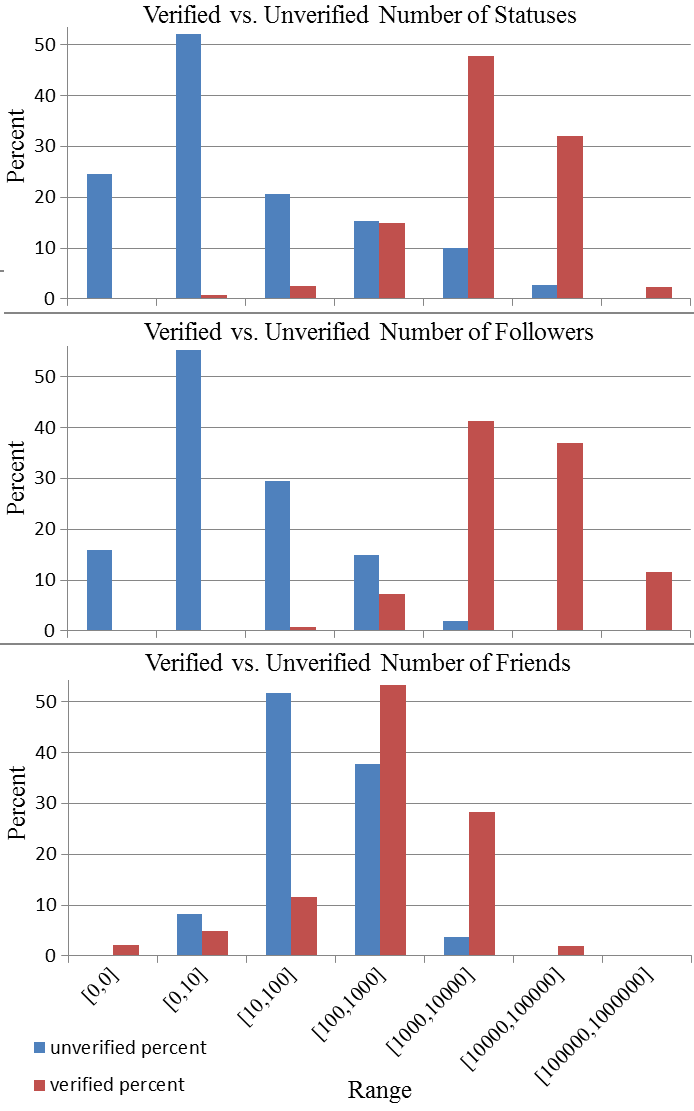
\includegraphics[width=4in]{Fig13.png}}
\caption[Verified vs. Unverified users]{Comparison of Verified vs. Unverified users using: (top) number of messages posted, (middle) total followers, and (bottom) total friends.}
\label{fig_ch7_7}
\end{figure}

Fig. \ref{fig_ch7_7} is a depiction using ranges from Table \ref{table_12_app2} differentiating verified vs. unverified over (i) the total number of messages (top chart), (ii) the total number of followers (middle chart), and (iii) the total number of friends (bottom chart). Fig. \ref{fig_ch7_7} bottom shows that a good portion of verified users is also engaged in following others (forming friend connections).

In summary, verified influencers are more likely to have more messages, more followers, and more friends. Given that most users are passive and do not generate much message traffic supports our argument for focusing on follower-followee link structure and profile metadata for mapping influence.

\section{Conclusions}
The social media site that is Twitter is a big data challenge. Twitter generates 500 million messages on a daily basis. It can be a daunting task to figure out how to collect the information that corresponds to the specific demographic of interest. This chapter presented a tool for quickly identifying influencers serving a specific demographic. This is important for content recommendation where we can identify influencers based on the composition of their audience using gender, ethnicity, language, location, or a combination of these. Also, by focusing on the followers of these influencers a community that is representative of the population of interest can be quickly established.

